\section{AWARE}\label{sec:aware}

\subsection{Image processing}
\label{img_proc}

As was noted in Sections 1 and 2, EUV waves are difficult to detect
since they are faint, extensive and propagate over a complex
background image (the solar corona). This realisation has driven past
attempts to enhance and detect EUV waves by making use of running
difference or base-difference images. However, these images, while
enhancing potential wavefronts, remain noisy and populated by other
extraneous features (see Figure \ref{rpdm_figure}). For AWARE, we therefore choose a different
approach, adopting a new, simple and very promising strategy for
segmenting an EUV wave wavefront from image data. Instead of using
traditional running- or base-difference image processing, we make use
of persistence imaging, as described by \citet{2014AAS...22421838T}.

A persistence image is found by calculating the persistence value of
the emission at each pixel at all locations and times.  The
persistence value at time $t$ of a time series $f(t)$ is simply the
maximum value reached by that pixel in the time range $0\rightarrow
t$.  If at later times the pixel value increases, the persistence
value increases accordingly. If the pixel value decreases however, the
persistence value remains unchanged. Hence, a set of persistence maps
constructed from an image sequence will indicate the brightest values
yet achieved in that sequence at each $t$.  The persistence transform
$P(t)$ of the time-series $f(t)$ is defined as
\begin{equation}
\label{eqn:persisttransform}
P(t) = \max_{t'=0}^{t'=t}f(t').
\end{equation}
Figure \ref{fig:persistence} shows the result of the pesistence
transform applied to some simulated data.  By obtaining sets of
persistence images from input solar EUV image data, and performing a
running difference operation on these images, rather than the original
input data, we are able to substantially enhance the appearance of
propagating waves. This is because running difference persistence images (RDPIs) have two particularly desirable
properties when searching for EUV waves.  Firstly, only pixels that
brighten over previous values have a non-zero value in the running
difference of persistence images, while zero-value pixels correspond
to areas that did not increase in brightness. Hence, since an EUV wave
brightens neighboring pixels as it moves across the Sun, the RDPIs
isolate those brightening pixels.  In other words, the RDPIs isolate
the leading part of the wavefront that brightened new pixels.
Secondly, since much of the corona does not vary significantly during
an EUV wave, RDPIs show very little residual coronal structure distant
from the EUV, greatly simplifying the resulting images.

\begin{figure}
\begin{center}
\includegraphics[width=16cm]{persistence_explanation.pdf}
\caption{Example of the application of the persistence transform.  The
original data $f(t)$ is shown in blue, and its persistence transform
$P(t)$ is shown in green.}
\label{fig:persistence}
\end{center}
\end{figure}

\begin{figure}
\begin{center}
\includegraphics[width=16cm]{differences.pdf}
\caption{Imaging processing techniques applied to three EUV waves,
  from 2011 October 1 (left column), 2011 February 13 (center column),
  and 2011 February 15 (right column) respectively. The top row shows
  percentage base difference (PBD) images of each event at a selected
  time, the image processing method used by the CorPITA algorithm
  \citep{2014SoPh..289.3279L}, while the second row shows the standard running
  difference (RD) images for these events (used in NEMO analysis,
  \citep{2005SoPh..228..265P}). In the bottom row, we show that the
  application of running difference persistence images (RDPI) as used
  by AWARE is able to extract the propagating EUV wave much more
  cleanly. Both Wave B and Wave C were analyzed in
  \cite{2014SoPh..289.3279L}; see their Fig. 7 and 8a respectively.}
\label{rpdm_figure}
\end{center}
\end{figure}

Figure \ref{rpdm_figure} illustrates the power of RDPIs for three
example EUV wave events from 2011 October 1 (Wave A), 2011 February 13
(Wave B), and 2011 February 15 (Wave C) respectively. For each event,
percentage base difference images (top row), running difference images
(center row) and RDPIs (bottom row) are shown. Waves B and C from
Figure \ref{rpdm_figure} were also analyzed by CorPITA in the
demonstration of that algorithm by \citet{2014SoPh..289.3279L}.  The
first row shows percentage base difference (PDB) images of each event,
the basic image type analyzed by the CorPITA algorithm.  The second
row shows running difference (RD) images, the basic image type
analyzed by the NEMO algorithm.  The third row shows RDPI images, the
basic image type analyzed by AWARE. Comparison with RDPIs shows that
in standard RD or PBD images the wavefront is more diffuse, and much
coronal structure not associated with the wavefront remains in the
image. RD and PBD images also have much denser noise compared to the
RDPIs of the same data; hence, separating the EUV wave from the noise
is substantially easier when using RDPIs.

Thus, the RPDI approach is the first step in the detection of EUV
waves with AWARE. Subsequent image processing steps allow us to refine
the detection of any propagating features. The major steps in the
AWARE detection and processing algorithm are described below, and are
demonstrated in Figure \ref{method_figure}.

\begin{enumerate}

\item Given a set of sequential solar EUV images (e.g. SDO/AIA or
  STEREO/EUVI data), data are summed in time and space to increase the
  signal to noise ratio of the wave against the background. Images may be summed in space as desired, for example an AIA image may be binned using $4\times4$ super-pixels to form $1024\times1024$ pixel images. In the time dimension, images may be summed as required. Typically, pairs or triplets of consecutive images are used.

\item The persistence transform is then applied to the resulting image
  set.  This creates a set of persistence images, showing the
  brightest values obtained in each pixel (see Equation
  \ref{eqn:persisttransform}) as a function of time.

\item Perform a running difference operation on the
  persistence images. Hence, only areas that increase in brightness
  from one time to the next remain (Figure \ref{method_figure}b).

\item Apply a noise reduction filter (Figure \ref{method_figure}c).
  Our demonstration algorithm uses a simple two step process.
  Firstly, all pixel values above a certain threshold are set to
  zero. This filters out spikes in the data. Secondly, a median filter
  with scale size $L=11$ image pixels is applied.  This replaces every
  pixel in the image with the median value found in its neighborhood,
  a disk of radius $L$ pixels.

\item Apply a morphological closing \citep{2002dip..book.....G}
  operation to every frame in the movie (a disk with radius $L$
  pixels).  This operation helps close small ‘cracks’ in structures
  \citep{2002dip..book.....G}.  The final image is shown in Figure
  \ref{method_figure}d.
\end{enumerate}

The final product is therefore a time-ordered series of images that
localize the bright wavefront of the EUV wave. Figure
\ref{method_figure} shows each step in this procedure, applied to two
AIA 211 $\AA$ images during the EUV wave event of 2011 October 1 (Wave
A in Figure \ref{rpdm_figure}). The result of the key step of
generating an RDPI (Steps 2 and 3) from the two input images is
illustrated in panel b). Steps 4 and 5 of the AWARE image processing
method (Figure \ref{method_figure}c, d) apply some basic noise
reduction and feature enhancement techniques with the intent to
further isolate the wave front in the data. The morphological closing operation is analagous to the automatic behaviour of the human eye, which is adept at smoothing over small-scale noise to identify a single coherent structure.

\begin{figure}
\begin{center}
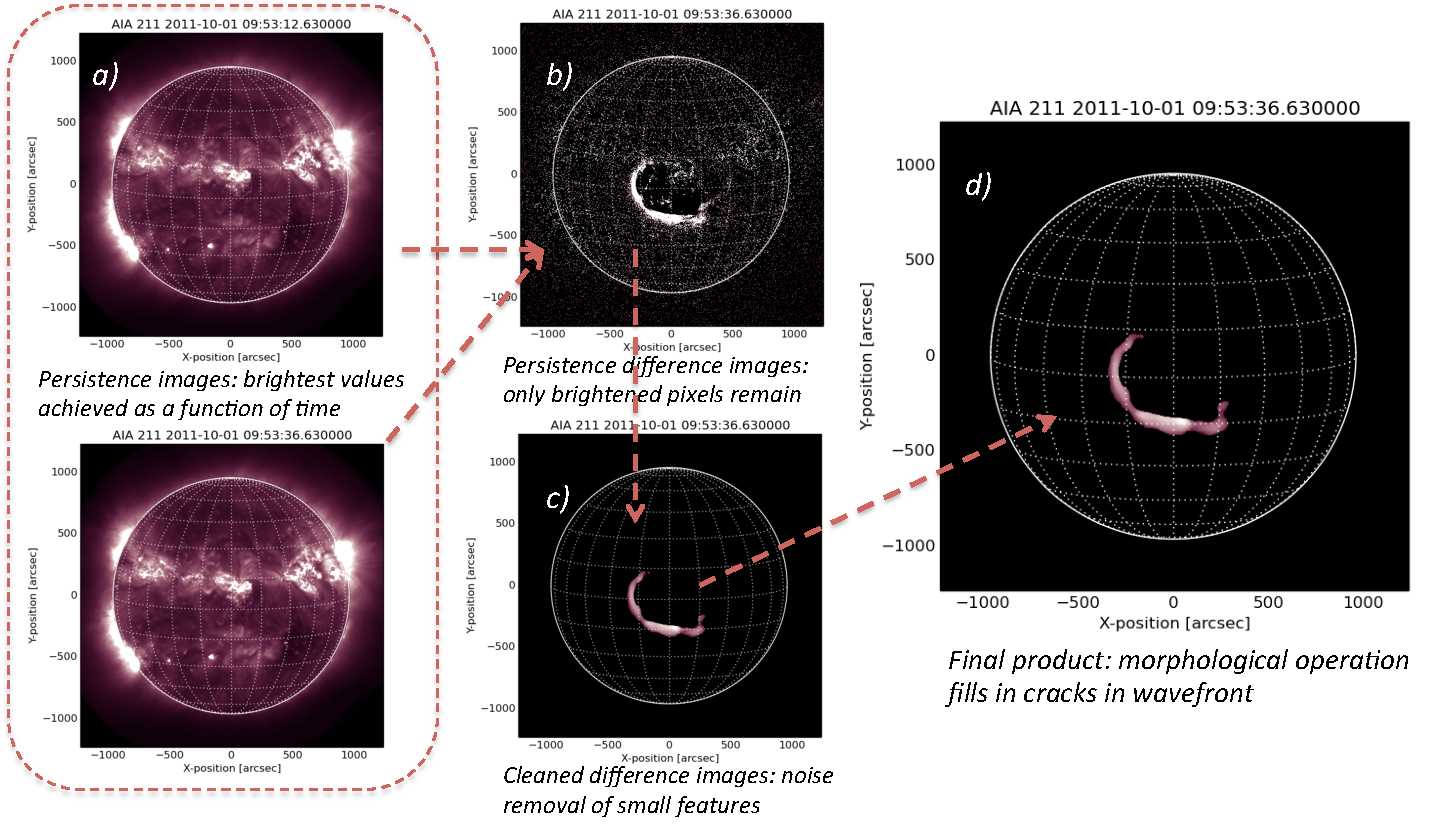
\includegraphics[width=16cm]{aware_figure4.pdf}
\caption{Example application of the AWARE image processing
  method. Panel a) shows two AIA 211$\AA$ images at different times
  during an EUV wave event. Panel b) illustrates the result of
  generating a running difference persistence image (RDPI) from the
  two input AIA images. The wavefront enhancement is evident. In panel
  c) a cleaning operation has been applied to the RDPI in order to
  remove small-scale features. Finally, in panel d) a morphological
  `closing operation' is applied, which has the effect of filling in
  small gaps in the detected wavefront
  \citep[e.g.][]{2002dip..book.....G}.}
\label{method_figure}
\end{center}
\end{figure}


The advantage of this approach is twofold. Firstly, we do not have to
fit a complex profile to noisy data in order to locate the
wavefront. Secondly, the RDPIs remove much more structure that is not
associated with a propagating bright front (Fig. 2, bottom row)
compared to the PBD images (Fig. 2, top-row), and therefore better
isolates the wavefront, making noise-cleaning easier (Fig. 4).  NEMO
\citep{2005SoPh..228..265P} uses integrals of annuli of RD images
(Fig. 2, middle row) to make their detections (Sec. 2.3). However, some
EUV waves do not propagate circularly (for example, wave A, Fig. 2)
and therefore the annular assumption can lead to a weakened detection.
Secondly, RD images contain dimming and brightening structure
unconnected with the EUV wavefront, and are noisier, when compared to
RDPIs, making isolation of the wavefront from these confounding
features more difficult. The final result of the first component of
AWARE is a time-series of images that may contain an EUV wave.  

\subsection{Wave characterization}
\label{wave_char}

The next step in the AWARE algorithm is to detect the presence of a wave, assess its
quality, and characterize its propagation through the solar
atmosphere. After the application of the image processing methods described in Section \ref{img_proc}, the next step in the detection and characterization process is to transform the solar image so that the  “north pole” of the new heliographic coordinate system is the estimated origin of the EUV wave. In these coordinates, a wave propagating uniformly across the Sun takes the form of an approximate straight line, with its velocity entirely in a southward direction [FIGURE EXAMPLE?].  This is the same transform as implemented by \citet{2014SoPh..289.3279L} and \citet{2005SoPh..228..265P}. This makes it easier to find and characterize propagating wavefronts.

The angular distance traversed at each image time is then estimated by taking cross-sections or `slices' of the transformed images and calculating the mean angular distance weighted by the intensity.  Error estimates are found by taking the standard deviation of the angular distance weighted by the intensity. These angular distances are fit with a quadratic equation to estimate the wave velocity and acceleration.

A propagating wave is determined to be present if we can measure its existence at at least one position along the wavefront, and at least two times: this is the minimum amount of information required to define a traveling feature.  CorPITA \citep{2014SoPh..289.3279L} use a quality score to assess how well determined is each part of the EUV wavefront. We adopt a similar apporach, with the intention of extending its usage to make it a powerful and simple tool to let the user decide what constitutes high and low quality EUV waves. For example, by adopting several indicators of the quality of the detection, the user may utilize the average and median scores to determine the overall quality of the event detection.  The minimum, maximum and standard deviation of the score lets the user determine the spread in the detection quality.  
